\documentclass[12pt, a4paper]{article}
\usepackage[utf8]{inputenc}
\usepackage{geometry}
\geometry{a4paper, margin=1in}
\usepackage{graphicx}
\usepackage{amsmath}
\usepackage{float}
\usepackage{hyperref}
\usepackage{caption}

\title{\textbf{Chaotic Oscillator}}
\author{
    \textbf{Name:} Yamulapalli Nandu Navadeep \\
    \textbf{Roll Number:} IMS24267 \\
    \textbf{Date of the Experiment:} August 24, 2026 \\
    \textbf{Date of Submission:} August 31, 2026
}
\date{}

\begin{document}

\maketitle

\section*{1. Name of the Experiment}
Chaotic Oscillator

\section*{2. Aim of the Experiment}
To explore the chaotic behavior of a driven nonlinear pendulum by graphing its motion in phase space and by making a Poincare plot, and to compare these plots to the motion of the pendulum when it is not chaotic. 

\section*{3. Theory}
The experimental setup consists of an aluminum disk connected to two springs. A point mass on the edge of the aluminum disk makes the oscillator nonlinear. This nonlinearity is required to cause chaotic motion. Furthermore, the disk is magnetically damped. 

Several quantities can be varied to cause regular, predictable motion to become chaotic. These variables are the driving frequency, driving amplitude, damping amplitude, and the initial conditions.

There are three different ways of plotting oscillations:
\begin{enumerate}
    \item \textbf{Angular Velocity ($\omega$) vs.\ Time ($t$)}
    \item \textbf{Phase Space:} Angular Velocity ($\omega$) vs.\ Angular Displacement ($\theta$)
    \item \textbf{Poincar\'e Plot:} Angular Velocity ($\omega$) vs.\ Angular Displacement ($\theta$) plotted only once per period of the driving force.
\end{enumerate}
The phase space and the Poincar\'e plot are particularly useful for recognizing chaotic oscillations. When the motion is chaotic, the graphs do not repeat.

\subsection*{Potential Well}
This pendulum has two equilibrium points, one on each side where the torque caused by the weight of the point mass is balanced by the torque from the springs. To map the potential energy $U$ versus the angular displacement $\theta$, the magnetic damping and the driving force are removed, and the pendulum is allowed to oscillate freely. 

By measuring the angular velocity, the kinetic energy $K$ is calculated. From the conservation of energy:
\[ \text{Total Energy} = U_i + K_i = U + K \]
Since the pendulum starts from rest at maximum displacement, $K_i = 0$, and:
\[ U_i = U + \frac{1}{2} I \omega^2 \]
As $U_i$ is a constant (let it be $c$), we have:
\[ U = c - \frac{1}{2} I \omega^2 \]
Therefore, the shape of the potential energy well can be found by plotting the negative of the square of the angular speed ($-\omega^2$) versus the angular displacement ($\theta$). The rotational inertia $I$ of the disk and point mass is calculated as:
\[ I = \frac{1}{2} M_{\text{disk}} R_{\text{disk}}^2 + M_{\text{pt mass}} R_{\text{disk}}^2 \]

\section*{4. Procedure}

\subsection*{Part I: Mapping the Potential Well}
\begin{enumerate}
    \item In PASCO Capstone, configured a graph of the potential energy ($U$) vs.\ angle.
    \item The driver power supply was turned off, and magnetic drag was minimized by moving the magnet away. The sensor was zeroed when the mass was at the top.
    \item The point mass was displaced to one side far enough that the disk would oscillate to the other side, then released to record the potential well.
\end{enumerate}

\subsection*{Part II: Resonant Frequency}
\begin{enumerate}
    \item Set up graphs of angular velocity vs.\ time and angular velocity vs.\ angle.
    \item The magnet was positioned about 3 mm from the disk for damping. The pendulum was displaced and allowed to oscillate without driving force to observe damped sinusoidal motion.
\end{enumerate}

\subsection*{Part III: Non-chaotic Oscillations}
\begin{enumerate}
    \item The driver arm amplitude was set to about 3.3 cm. The power supply was turned on at approximately 3.5 V to drive the system in a simple back-and-forth motion.
    \item Recorded the data to observe regular (non-chaotic) phase diagrams and Poincar\'e plots.
\end{enumerate}

\subsection*{Part IV: Chaotic Oscillations}
\begin{enumerate}
    \item Gradually increased the driving frequency by increasing the voltage on the power supply until the pendulum's motion became complicated (chaotic).
    \item Adjusted the magnet distance if necessary to keep from over-driving.
    \item Data was recorded for a longer duration to observe the chaotic motion in phase space, angular velocity vs.\ time, and the Poincar\'e plot. 
    \item An FFT of the angular velocity was also examined.
\end{enumerate}

\section*{5. Tabular Column}
As the data was continuously acquired using the PASCO Capstone interface via a Rotary Motion Sensor, large arrays of continuous time-series data were recorded. Consequently, a traditional manual tabular column is not applicable. The values were directly fed into the software to compute angular displacement and angular velocity.

\section*{6. Calculations}
Using the PASCO Capstone software's calculator, the potential energy is continuously mapped using:
\[ U = c - 0.5 \cdot I \cdot \omega^2 \]
where $c$ was arbitrarily set to 1, and $I$ was evaluated from the measured mass and radii of the disk and the point mass.

\section*{7. Results and 8. Graphs}

The experimental observations were captured digitally. The graphs clearly show the transition from regular motion to chaotic motion.

\subsection*{1. Potential Well}
The potential well exhibits a double-well structure corresponding to the two stable equilibrium points.
\begin{figure}[H]
    \centering
    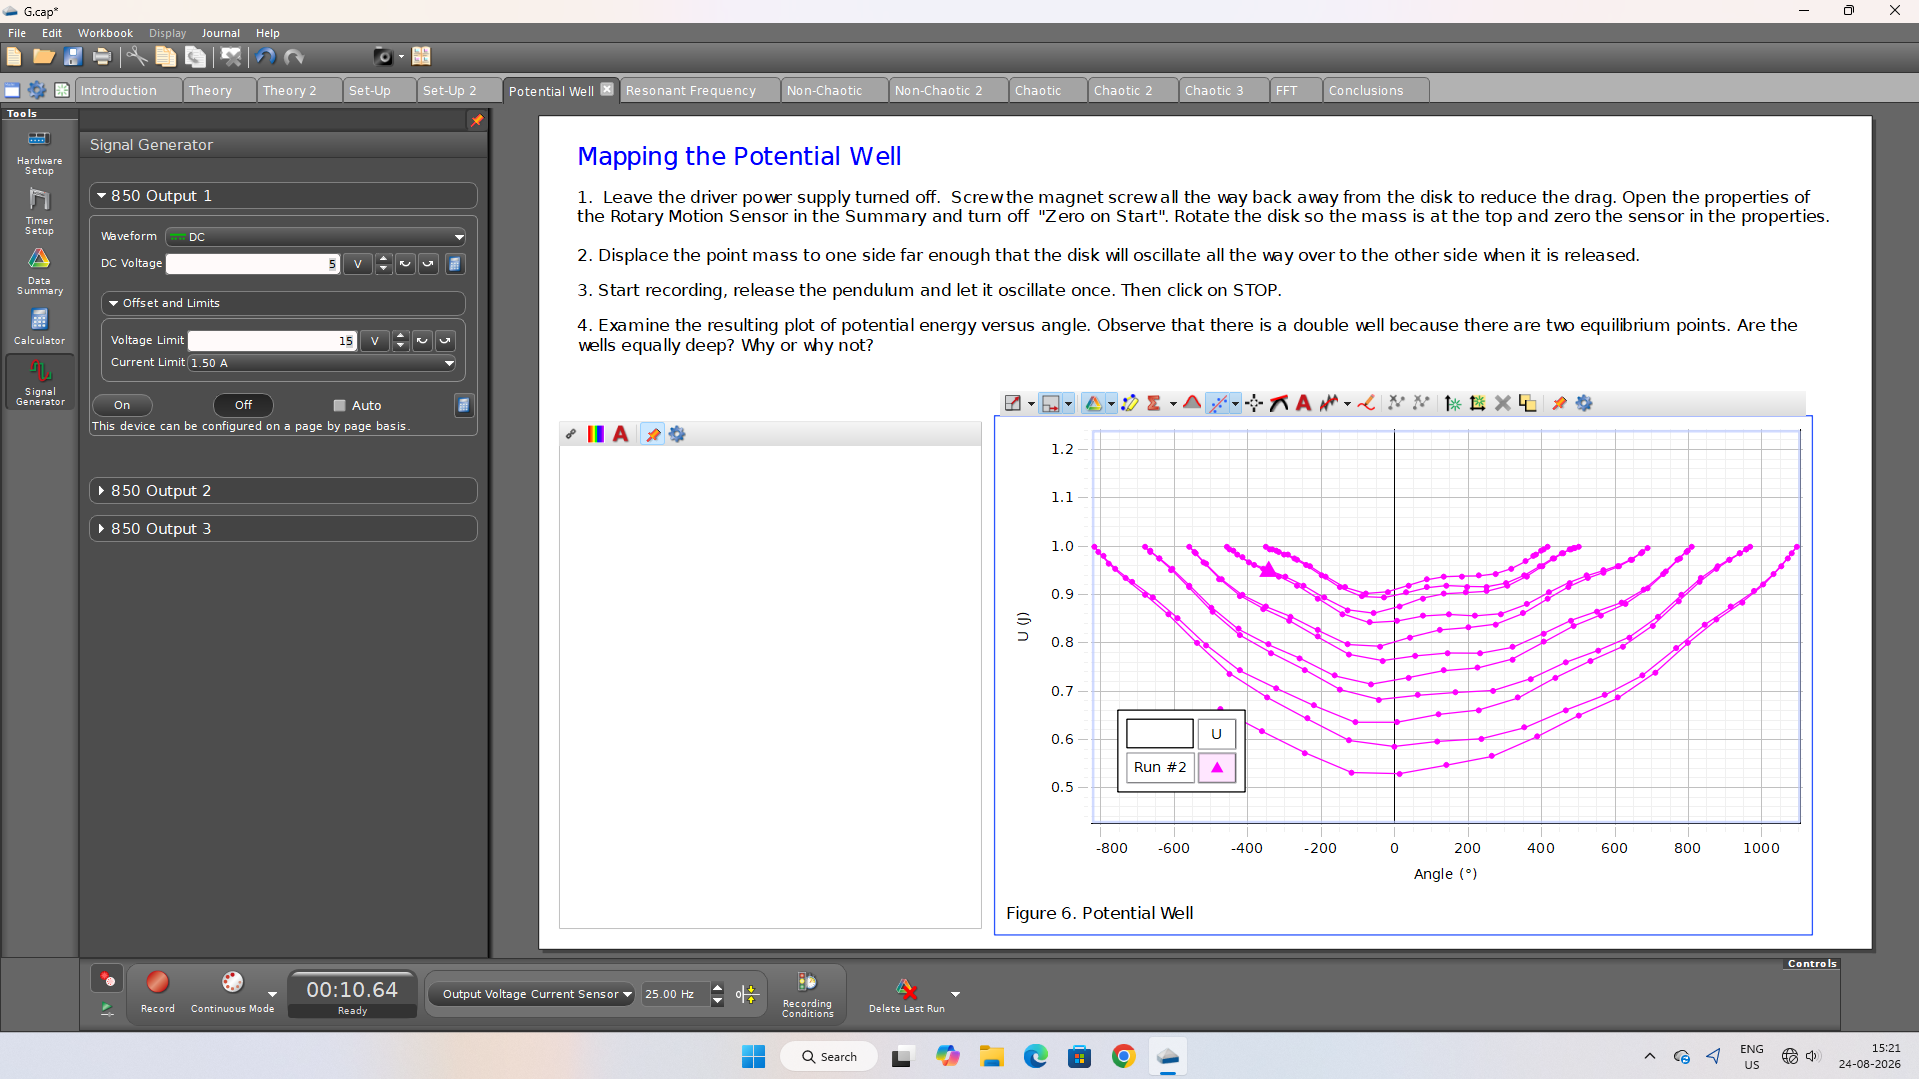
\includegraphics[width=0.8\textwidth]{exp-observations/potential well.png}
    \caption{Potential Well of the nonlinear oscillator.}
\end{figure}

\subsection*{2. Resonant Frequency (Damped Oscillations)}
Without a driving force, the pendulum shows damped oscillations towards one of the equilibrium points.
\begin{figure}[H]
    \centering
    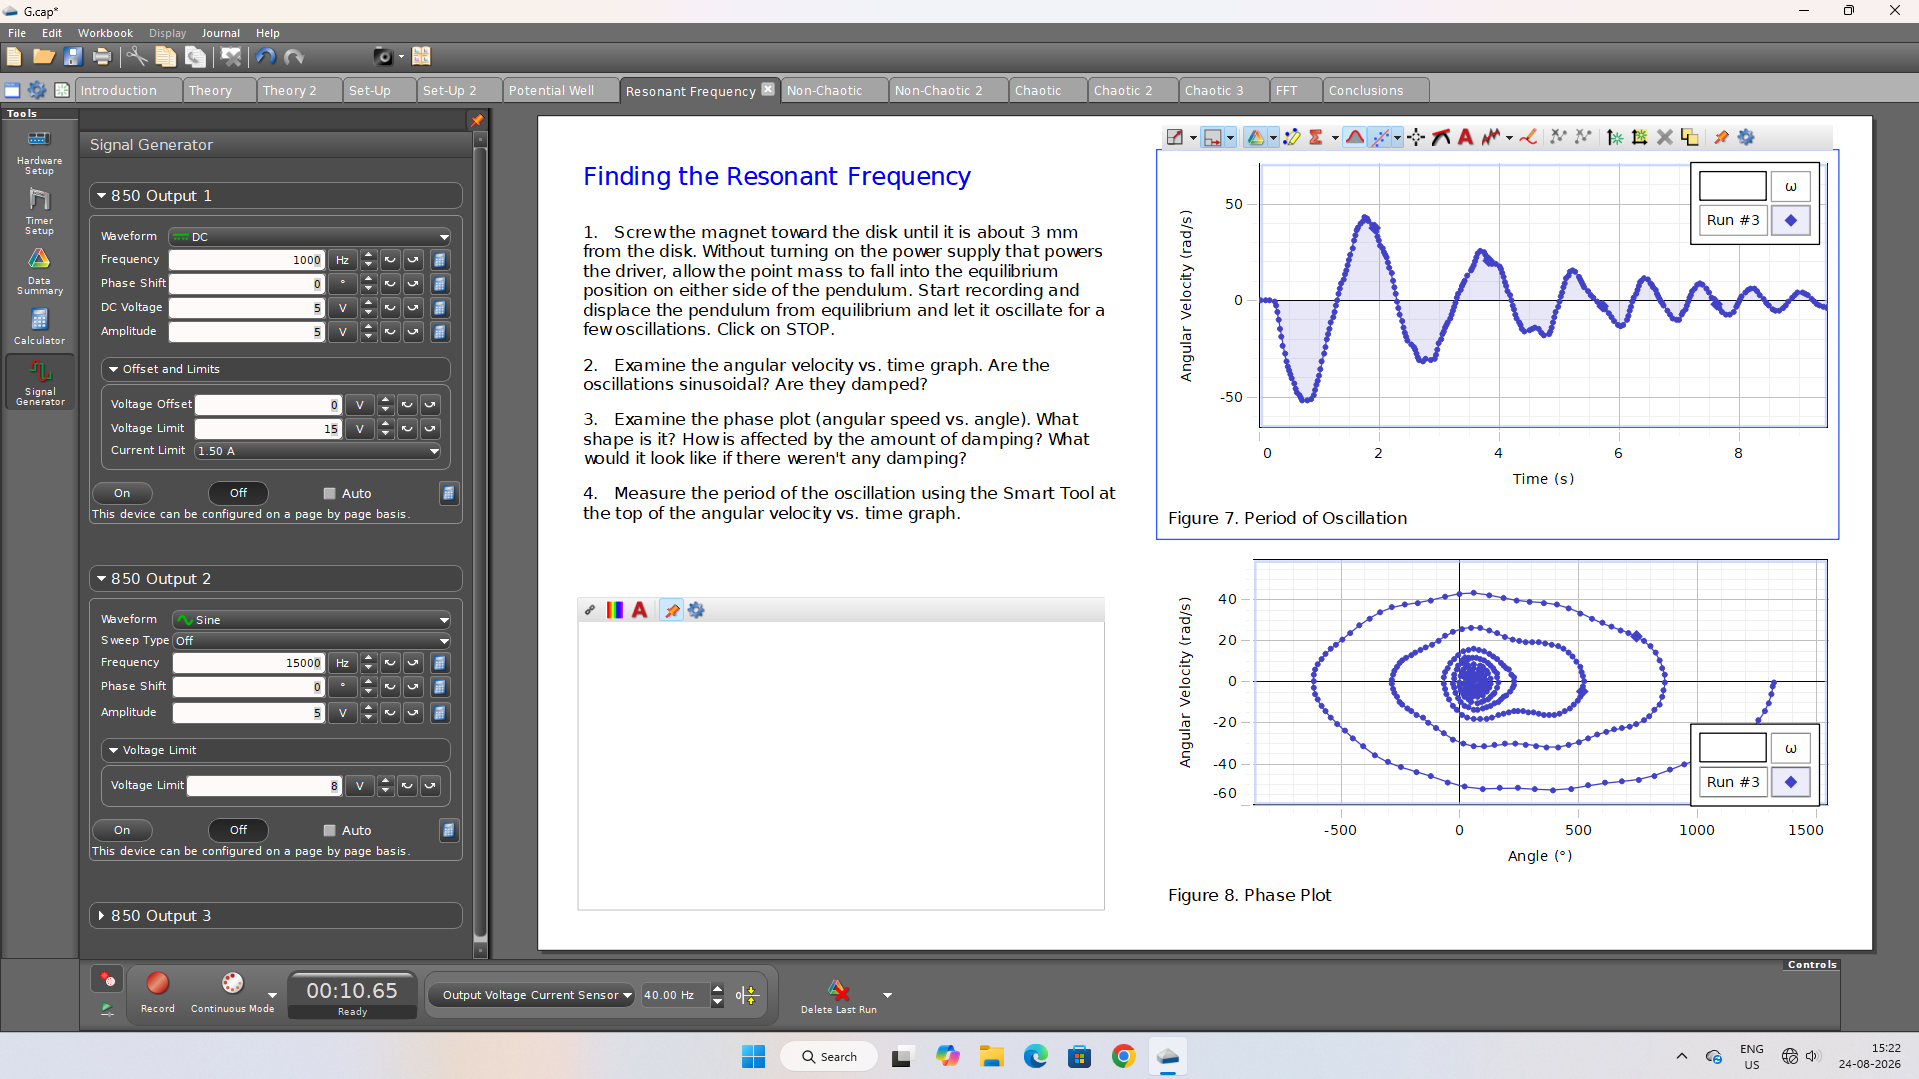
\includegraphics[width=0.8\textwidth]{exp-observations/resonant frequesncy.png}
    \caption{Angular velocity vs.\ time for damped oscillations.}
\end{figure}

\subsection*{3. Non-Chaotic Oscillations}
When driven at a steady, moderate frequency, the oscillator settles into a stable, repeating limit cycle.
\begin{figure}[H]
    \centering
    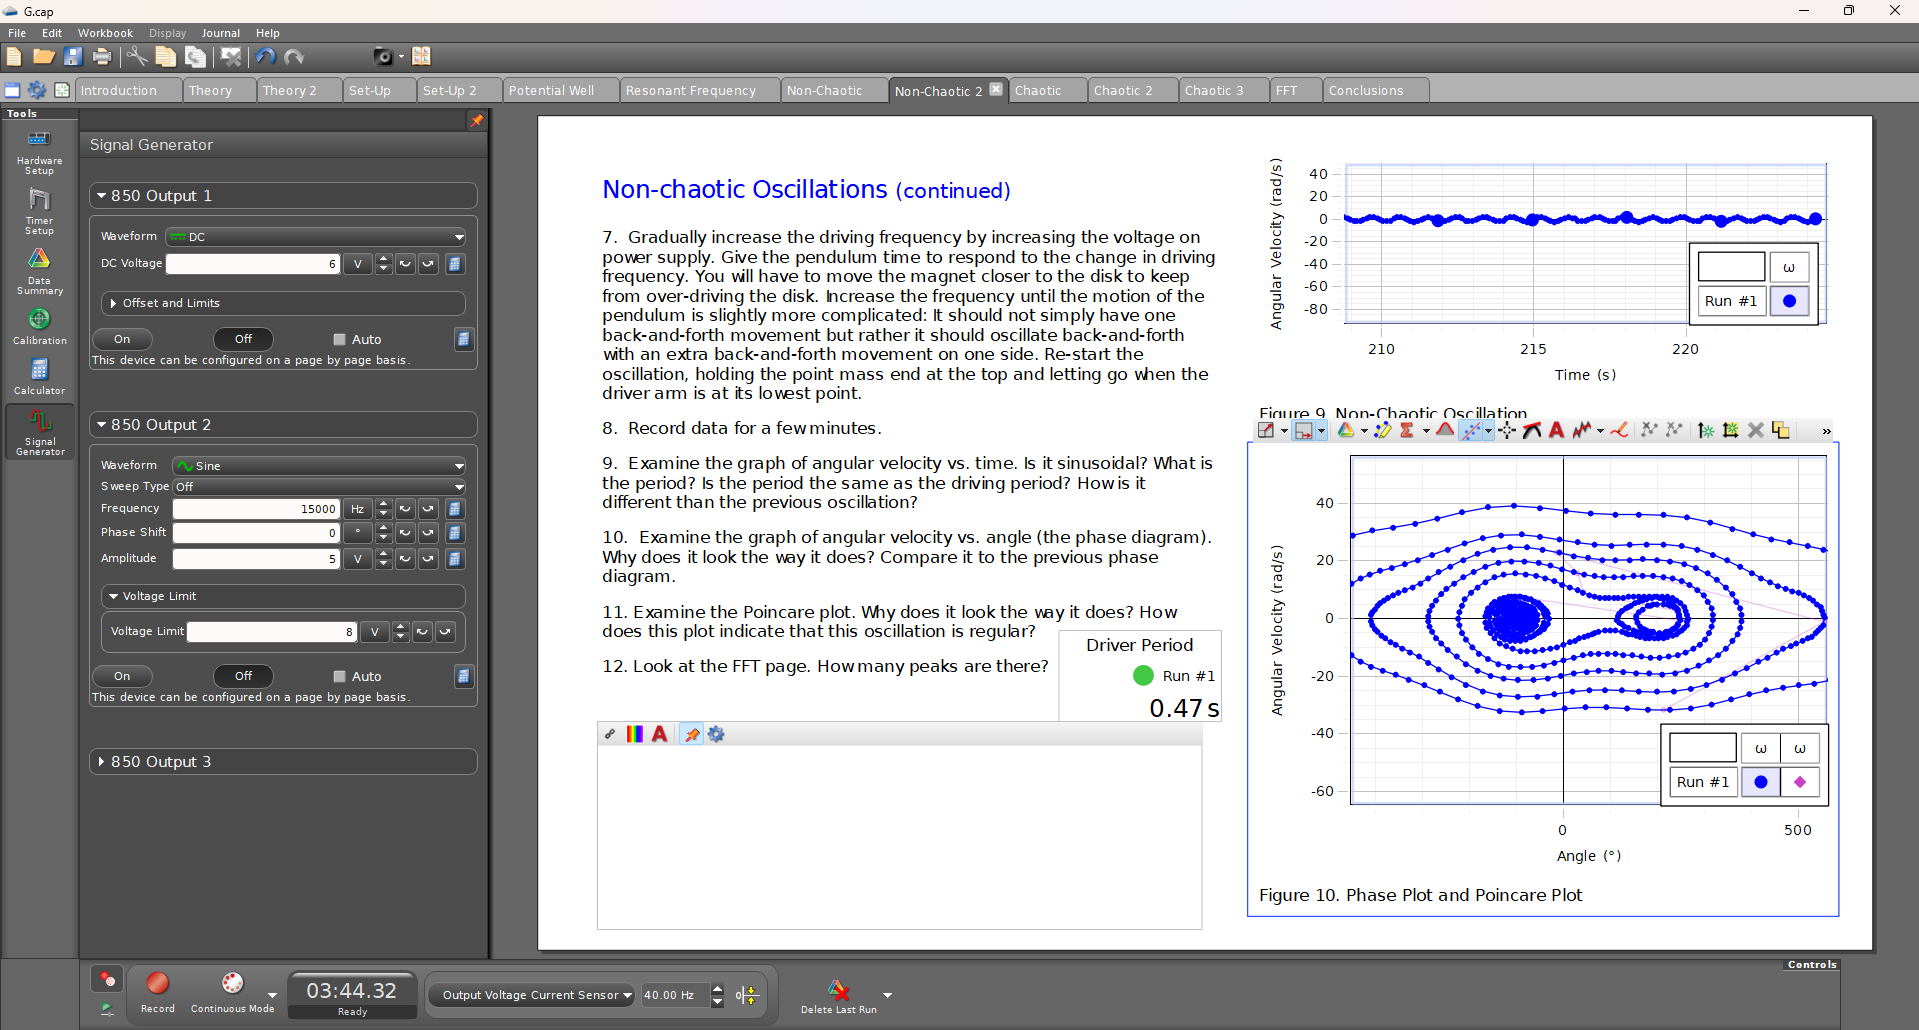
\includegraphics[width=0.8\textwidth]{exp-observations/Non-chaotic oscillations.png}
    \caption{Phase space and time-series for non-chaotic driven oscillations.}
\end{figure}

\subsection*{4. Chaotic Oscillations}
As the driving frequency is increased, the motion becomes unpredictable. The phase space trajectory does not close on itself, and the Poincar\'e section forms a strange attractor rather than a single point or finite set of points.
\begin{figure}[H]
    \centering
    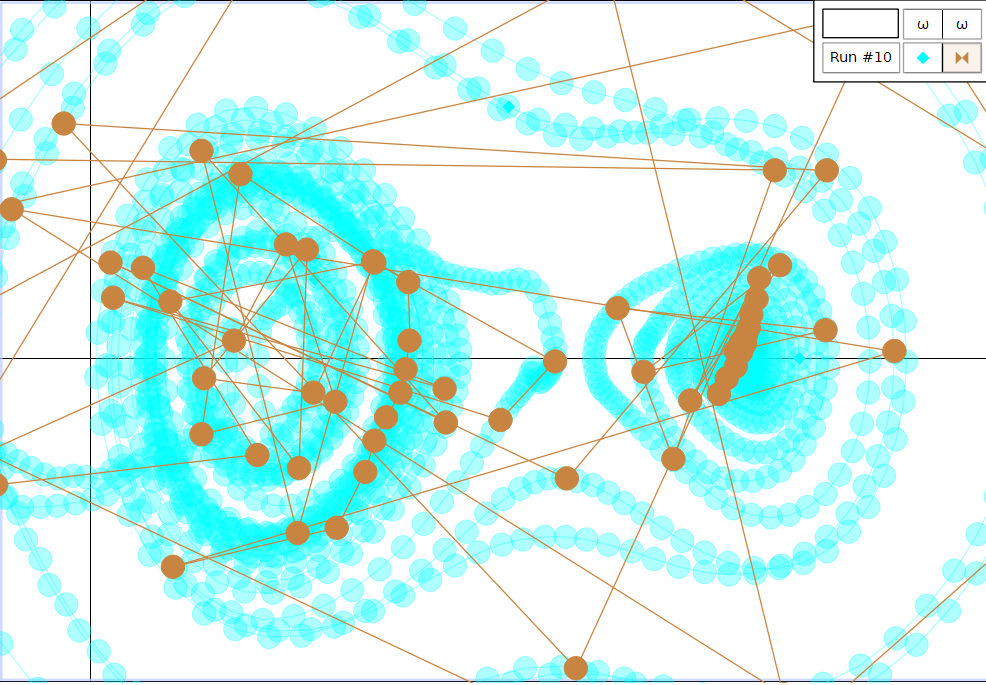
\includegraphics[width=0.8\textwidth]{exp-observations/chaotic1.png}
    \caption{Chaotic oscillations showing unpredictable transitions between the two potential wells.}
\end{figure}

\begin{figure}[H]
    \centering
    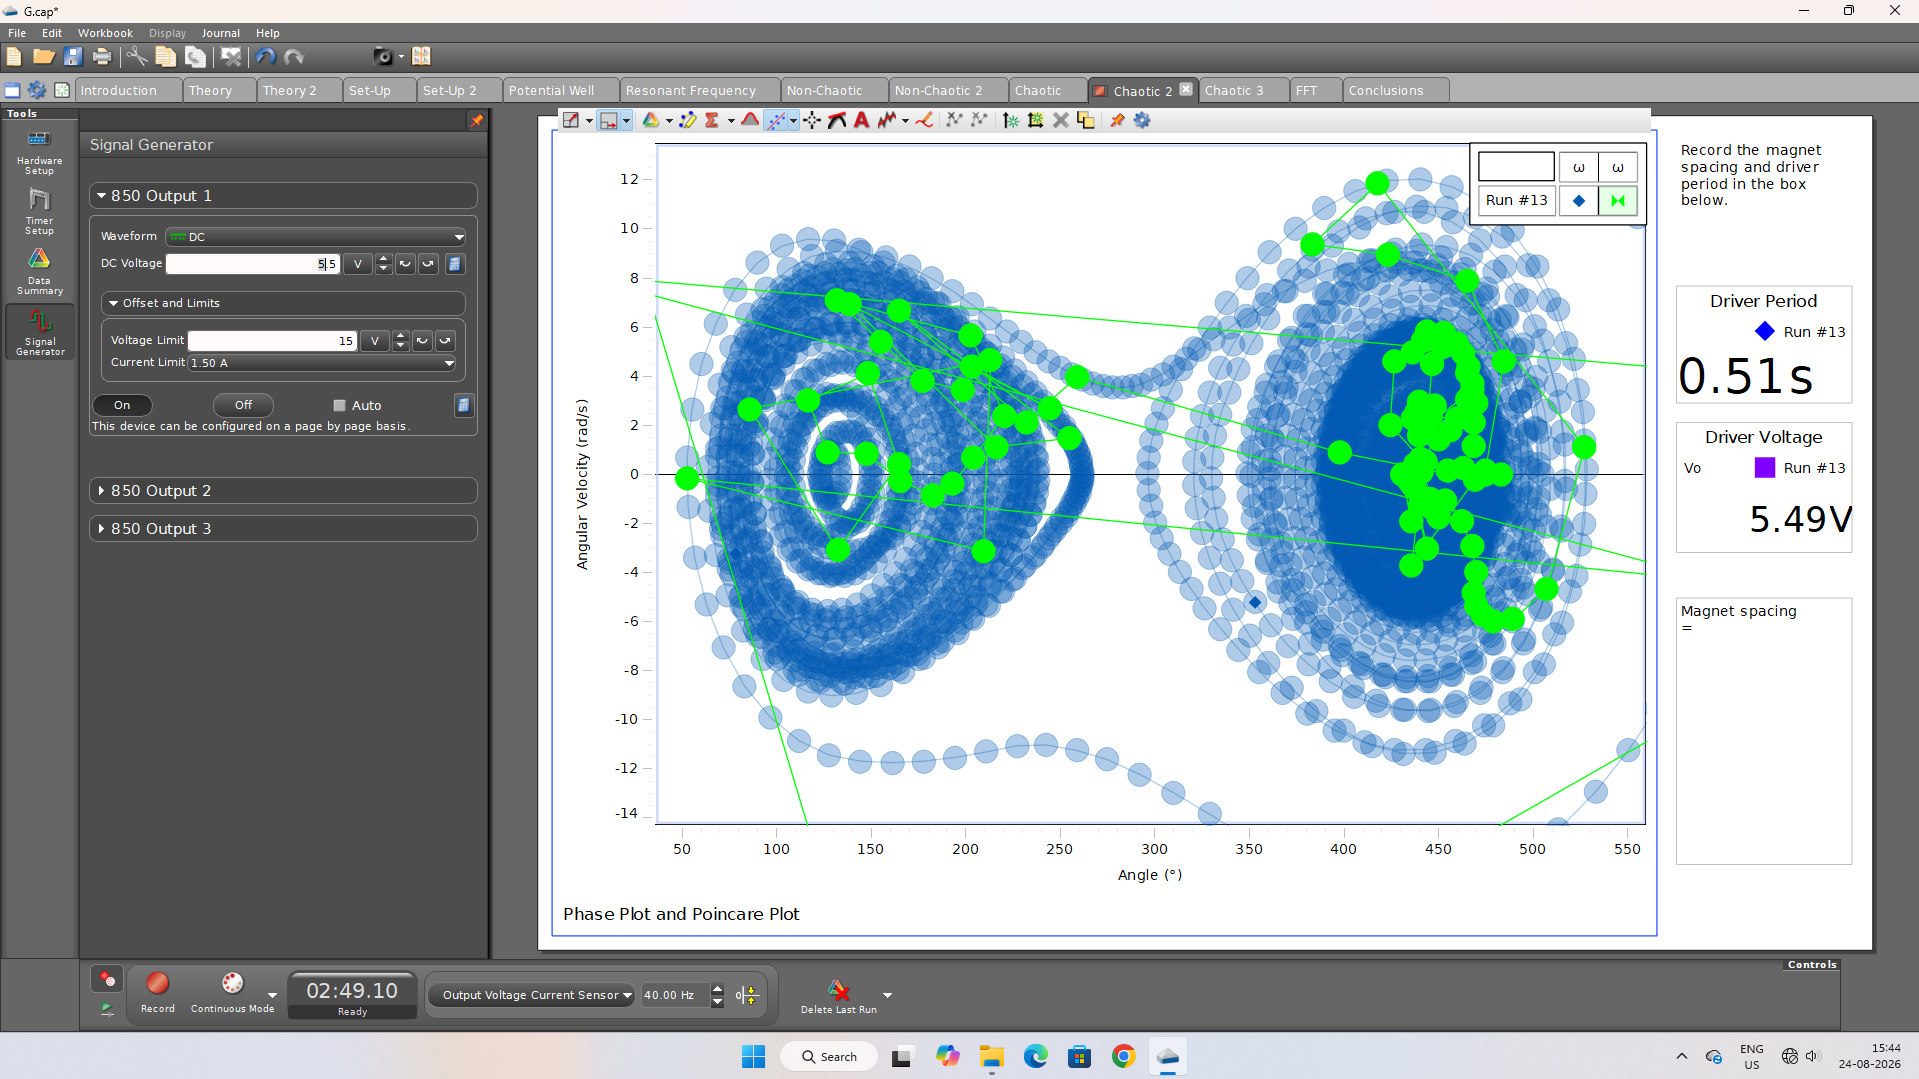
\includegraphics[width=0.8\textwidth]{exp-observations/chaotic2-phase plot.png}
    \caption{Phase plot of chaotic oscillations.}
\end{figure}

\begin{figure}[H]
    \centering
    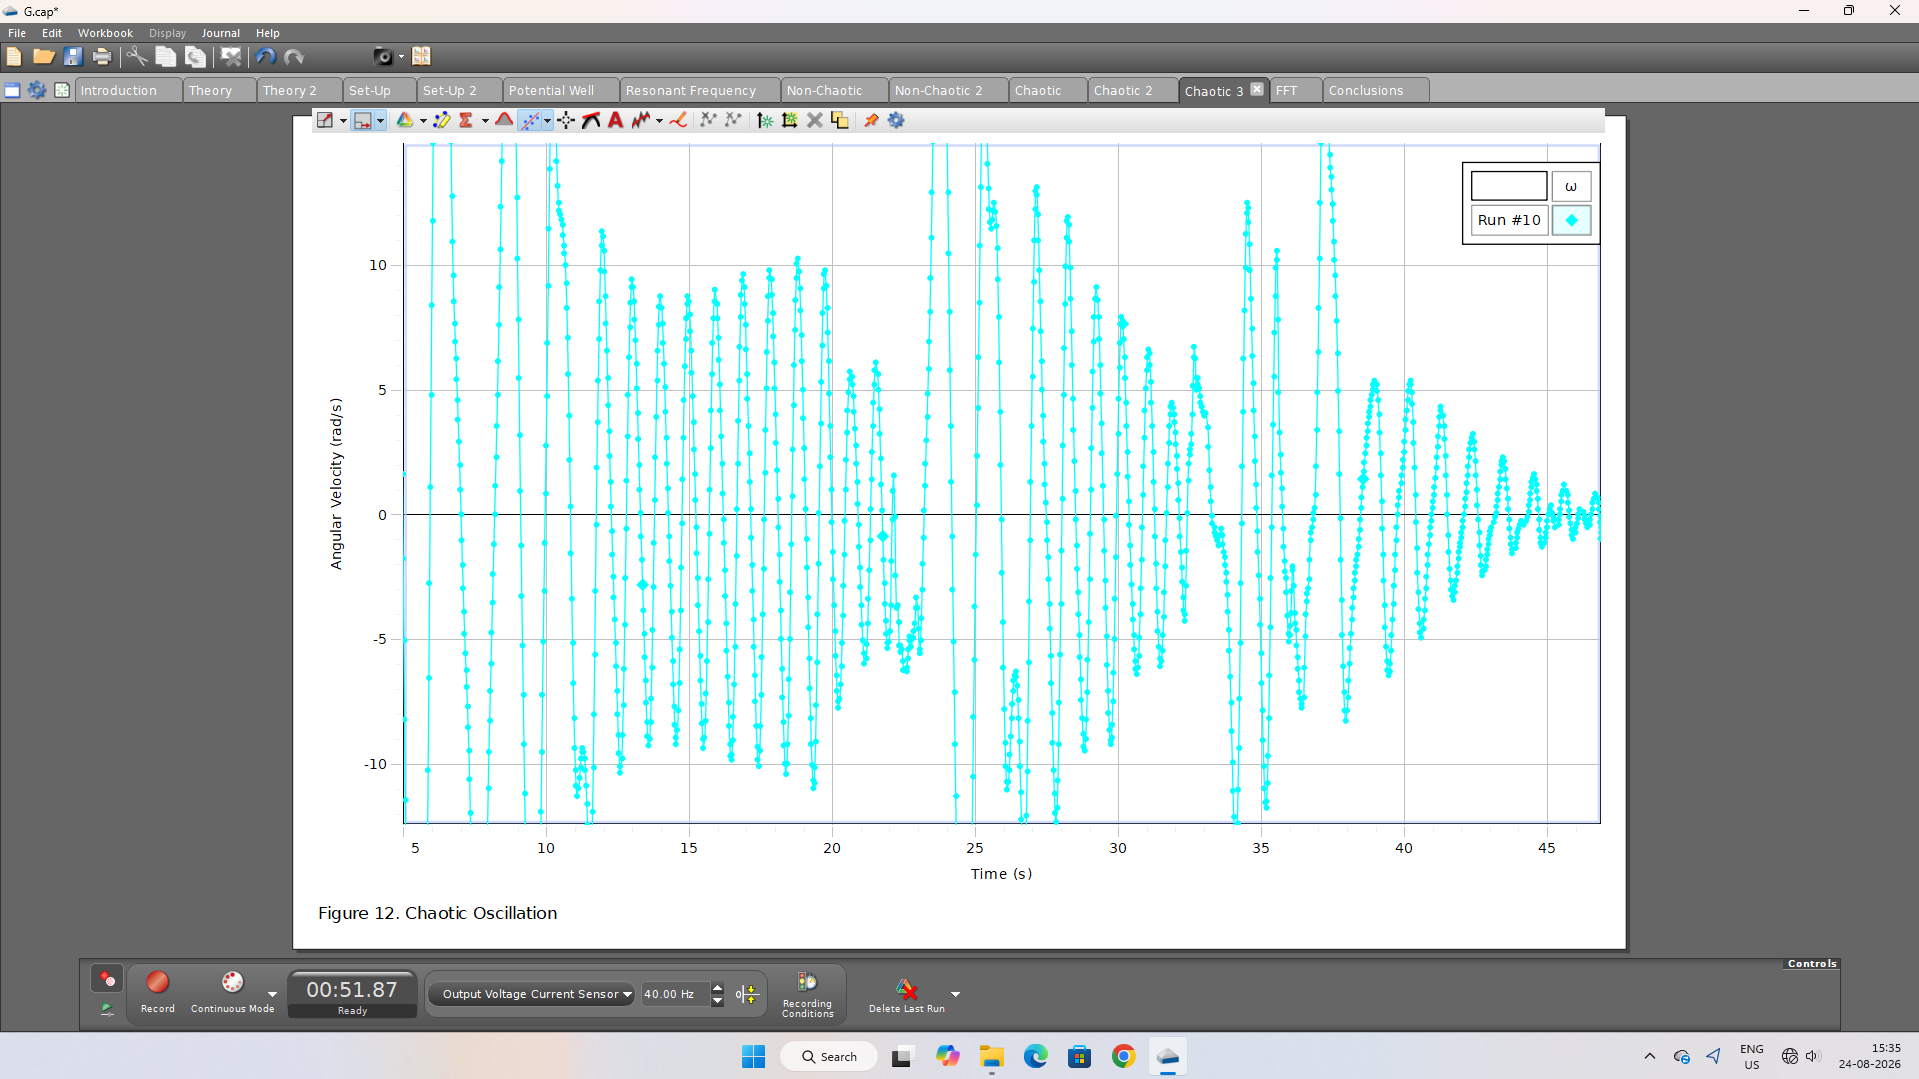
\includegraphics[width=0.8\textwidth]{exp-observations/Chaotic oscillation - w vs t.png}
    \caption{Angular velocity vs.\ time for chaotic oscillations.}
\end{figure}

\begin{figure}[H]
    \centering
    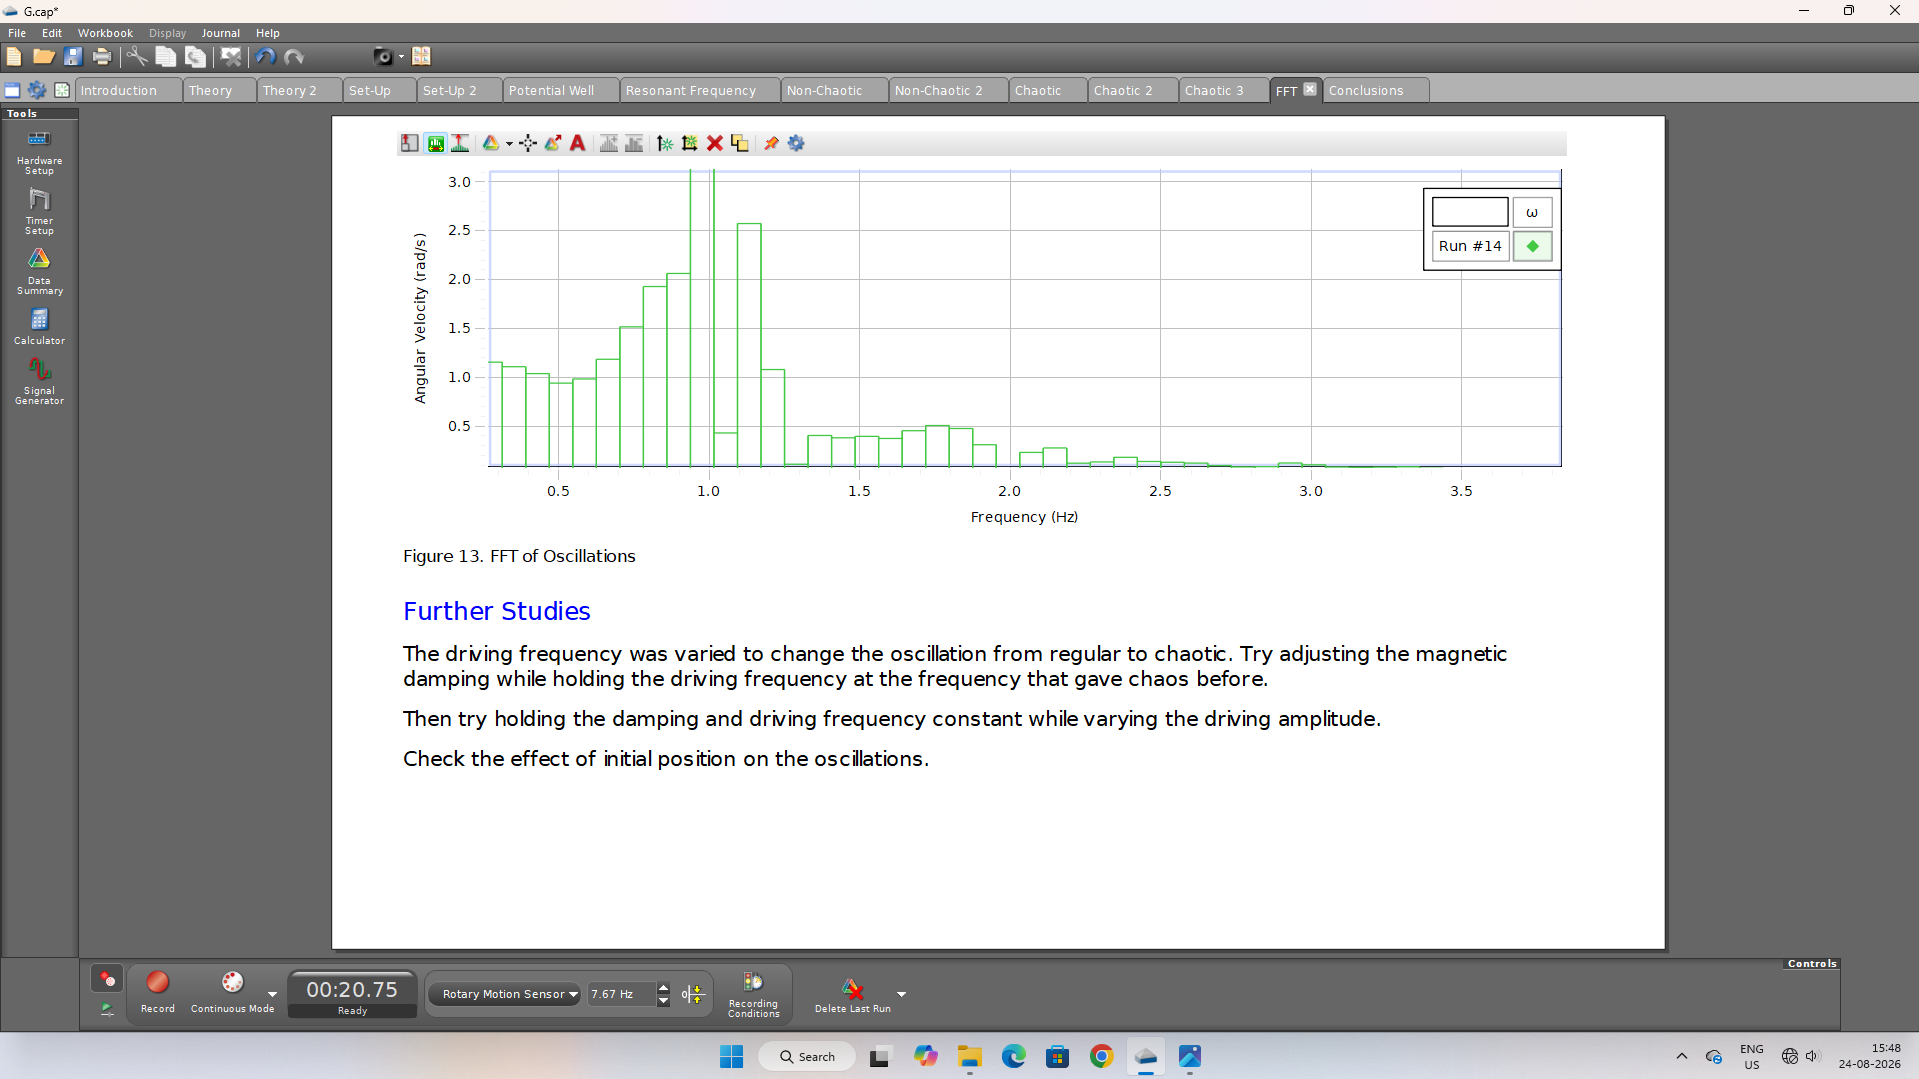
\includegraphics[width=0.8\textwidth]{exp-observations/FFT of oscillations.png}
    \caption{Fast Fourier Transform (FFT) of the chaotic oscillations, revealing a broad continuous spectrum typical of chaos.}
\end{figure}

\section*{9. Error Calculation}
The primary sources of error in this experiment include:
\begin{itemize}
    \item \textbf{Sensor Resolution:} The Rotary Motion Sensor has a finite angular resolution which introduces a small quantization error in the displacement and derived angular velocity.
    \item \textbf{Friction and Damping Variability:} Unaccounted friction in the bearings and slight variations in the magnetic damping (due to non-uniformity in the disk's thickness or composition) could affect the ideal assumptions.
    \item \textbf{Measurement of Inertia:} Minor inaccuracies in measuring the mass and radius of the point mass and the disk contribute to systemic errors in the calculation of $I$ and consequently $U$.
\end{itemize}
Because the purpose of the experiment is primarily qualitative observation of nonlinear dynamics and mapping phase space topologies (attractors, Poincar\'e sections), these quantitative errors do not detract from the identification of chaotic regimes.

\section*{10. Discussion}
The experiment successfully demonstrated the behavior of a nonlinear driven oscillator and its transition from periodic motion to deterministic chaos. Initially, the potential energy curve mapping confirmed the double-well nature of the system, which arises because the gravitational torque on the point mass competes with the restoring torque of the springs. 

In the regular driven regime, the pendulum oscillates back and forth within a predictable cycle. Its phase plot shows a closed loop (a limit cycle), indicating periodic behavior. However, upon changing the driving frequency, the system undergoes bifurcations leading to chaos. 

During chaotic oscillation, the pendulum's motion becomes highly sensitive to initial conditions. It may oscillate a few times in one well and then suddenly gain enough energy to cross the central potential barrier into the other well, seemingly at random. The phase plot becomes a complex, non-repeating web (a strange attractor). The FFT of the chaotic regime shows a broad spectrum of frequencies, unlike the discrete sharp peaks seen in periodic motion. 

The main difference between the theoretical assumptions and the real-life setup is that theoretical models often assume perfect linearity in the springs and completely uniform damping. In real life, the magnetic drag might vary slightly depending on the exact position of the disk, and the springs might exhibit slight non-ideal behaviors. Nevertheless, the characteristic signature of chaos—broadband FFT, non-repeating phase trajectories, and complex Poincar\'e plots—was unmistakably observed.

\section*{11. References}
\begin{enumerate}
    \item PASCO Scientific, \textit{Chaos EX-5523 Equipment Manual}.
    \item Thornton, S. T., \& Marion, J. B. (2003). \textit{Classical Dynamics of Particles and Systems}. Brooks/Cole.
    \item Strogatz, S. H. (2014). \textit{Nonlinear Dynamics and Chaos: With Applications to Physics, Biology, Chemistry, and Engineering}. Westview Press.
\end{enumerate}

\end{document}
